%%%%%%%%%%%%%%%%%%%%%%%%%%%%%%%%%%%%%%%%%%%%%%%%%%%%%%%%%%%%%%%%%%%%%%%%%%%%%%%%
%2345678901234567890123456789012345678901234567890123456789012345678901234567890
%        1         2         3         4         5         6         7         8

\documentclass[letterpaper, 10 pt, conference]{ieeeconf}  % Comment this line out
                                                          % if you need a4paper
%\documentclass[a4paper, 10pt, conference]{ieeeconf}      % Use this line for a4
                                                          % paper

\IEEEoverridecommandlockouts                              % This command is only
                                                          % needed if you want to
                                                          % use the \thanks command
\overrideIEEEmargins
% See the \addtolength command later in the file to balance the column lengths
% on the last page of the document



% The following packages can be found on http:\\www.ctan.org
%\usepackage{graphics} % for pdf, bitmapped graphics files
%\usepackage{epsfig} % for postscript graphics files
%\usepackage{mathptmx} % assumes new font selection scheme installed
%\usepackage{times} % assumes new font selection scheme installed
%\usepackage{amsmath} % assumes amsmath package installed
%\usepackage{amssymb}  % assumes amsmath package installed
\usepackage[utf8]{inputenc}
\usepackage[spanish]{babel}
\usepackage{amsfonts}

\usepackage{graphicx}

\title{\LARGE \bf
Teoría de las Comunicaciones: Trabajo Práctico 1
}

%\author{ \parbox{3 in}{\centering Huibert Kwakernaak*
%         \thanks{*Use the $\backslash$thanks command to put information here}\\
%         Faculty of Electrical Engineering, Mathematics and Computer Science\\
%         University of Twente\\
%         7500 AE Enschede, The Netherlands\\
%         {\tt\small h.kwakernaak@autsubmit.com}}
%         \hspace*{ 0.5 in}
%         \parbox{3 in}{ \centering Pradeep Misra**
%         \thanks{**The footnote marks may be inserted manually}\\
%        Department of Electrical Engineering \\
%         Wright State University\\
%         Dayton, OH 45435, USA\\
%         {\tt\small pmisra@cs.wright.edu}}
%}

\author{Axel Straminsky, Jorge Quintana, Florencia Zanollo, Luis Toffolleti}% <-this % stops a space



\begin{document}

\maketitle
\thispagestyle{empty}
\pagestyle{empty}


%%%%%%%%%%%%%%%%%%%%%%%%%%%%%%%%%%%%%%%%%%%%%%%%%%%%%%%%%%%%%%%%%%%%%%%%%%%%%%%%
\begin{abstract}
En el presente trabajo se utilizan la libreria Scapy de Python y la herramienta Wireshark para capturar paquetes ARP en varias redes y modelar dos fuentes de memoria nula. Sobre estas fuentes se efectúa un análisis de la entropía de cada una de ellas y de la cantidad de información que transmite cada símbolo de estas fuentes. Adicionalmente se busca verificar qué datos de la topología de las redes subyacentes pueden descubrirse en base a los símbolos distinguidos de estas fuentes y ayudar a la profundización del conocimiento sobre el protocolo ARP en escenarios reales.
\end{abstract}
\begin{keywords}
ARP, Scapy, Wireshark, Entropía, Fuentes de memoria nula, Cantidad de información, Topología de redes en capa 2.
\end{keywords}

%%%%%%%%%%%%%%%%%%%%%%%%%%%%%%%%%%%%%%%%%%%%%%%%%%%%%%%%%%%%%%%%%%%%%%%%%%%%%%%%
\section{Introducción}

%El objetivo de este trabajo es analizar diversos aspectos de una red como su topología, y otros aspectos más teóricos como la entropía y la información de cada nodo. Para realizar este análisis modelamos los paquetes capturados como dos fuentes de memoria nula $S$ y $S1$, las cuáles tienen como símbolos los paquetes ARP broadcast y unicast, en el caso de $S$, y las direcciones IP de destino de estos paquetes en el caso de $S2$.

El objetivo del presente trabajo es descubrir la topología de distintas redes utilizando captura de paquetes ARP. Para la clasificación de los datos así obtenidos se modelaran por cada red dos fuentes de memoria nula, que identificaremos como $S$ y $S1$. Para las fuentes $S$ se distinguirán los paquetes broadcast vs. los paquetes unicast y para las fuentes $S1$ los símbolos se distinguirán basados en las direcciones IP de los orígenes de los paquetes.

ARP es un protocolo de capa 2.5 que se encarga de traducir direcciones IP (Nivel de red) a direcciones físicas de los dispositivos o ''MAC addresses'' (Nivel de Enlace). Este protocolo distingue dos tipos de mensajes, ''Who has'' y ''Is At''.
''Who has'' son típicamente mensajes de ''pedido'' (request) enviados a toda la red (Broadcast) preguntando a los dispositivos, identificados por MAC address, quién poseé cierta dirección IP.
''Is At'' son mensajes de ''respuesta'' (reply) enviados a un sólo nodo (unicast) que es el nodo que efectuó el pedido, indicando que el dispositivo con la IP buscada se encuentra en la dirección física que envia la respuesta.

Un dispositivo comunicándose en una red a nivel capa de enlace, necesita conocer la dirección MAC del dispositivo con el que desea comunicarse, pero el protocolo IP utiliza direccionamiento por dirección IP. Para traducir de un tipo de direccionamiento al otro de manera eficiente, los dispositivos mantienen una tabla ARP que ''cachea'' la información. Estas tablas ARP son actualizadas cada cierto tiempo, lo que genera los mensajes de protocolo ARP que capturaremos.

La distinción entre tipos de paquetes que soporta el protocolo ARP nos conduce de forma natural a la primera distinción entre símbolos que utilizaremos para modelar la fuente $S$, que distinguirá entre paquetes de tipo Broadcast y paquetes de tipo Unicast.


Para el modelado de la fuente $S1$ el criterio de distinción entre los símbolos de la fuente se justifica  matemáticamente de acuerdo a la cantidad de información que cada símbolo trae aparejado y su comparación con la entropía total del sistema.

La cantidad de información que aporta un evento $E$ que ocurre con probabilidad $P(E)$ se define como 
\[I(E) = log \frac{1}{P(E)}\]

Para calcular la cantidad promedio de información de una fuente de memoria nula $S$, tenemos que cuando el simbolo $s_i$ ocurre, obtenemos una cantidad de información 
\[I(s_i) = log \frac{1}{P(s_i)}\]
y la probabilidad de que esto ocurra es directamente $P(s_i)$ con lo cual la cantidad promedio de información por cada símbolo de la fuente $S$ será
\[H(S) = \sum_{S} P(s_i) I(s_i)\]

A esta cantidad se la conoce como la entropía de la fuente $S$: $H(S)$.

La primera conclusión que se puede sacar de la definición es que los eventos que más información aportan son aquellos con menor probabilidad de ocurrir.

Es claro que en nuestro modelo no estamos trabajando con fuentes de memoria nula ideales, sino que estamos utilizando redes reales para modelar las mismas, con lo cual las probabilidades serán en realidad estadísticos obtenidos en base a la experimentación (captura de paquetes). Los estadísticos utilizados serán el ratio entre la cantidad de ocurrencias de un evento y el total de los eventos capturados, por esta razón y con la intención que el estadístico sea representativo de la probabilidad de ocurrencia de los eventos se efectuarán capturas durante intervalos de tiempo mayores a diez minutos.

%Para complementar el análisis se estudiará la entropía de las fuentes modeladas y se analizará la cantidad de información inherente a cada uno de sus simbolos, con esto buscamos justificar el criterio de distinguibilidad de los mismos



\section{Desarrollo}
%Para realizar este TP utilizamos como herramientas Wireshark[1], Scapy[2], y Python. 
Para el presente trabajo práctico se desarrolló un programa en Python utilizando la libreria Scapy que captura los paquetes que escucha la interfaz definida y filtra los mismos quedandose solamente con aquellos que son paquetes del protocolo ARP, el mismo programa acepta como parámetros la ruta de un archivo en formato ''.pcap'' que puede ser generado por medio de capturas anteriores o utilizando software alternativo como Wireshark.

Distintas variantes del programa permiten clasificar los paquetes capturados de acuerdo a la distinción entre paquetes con direccionamiento Broadcast o direccionamiento Unicast así como distinguiendo por direcciones IP de origen para modelar las fuentes $S$ y $S1$ respectivamente. Con estos datos se calculan la entropía y la cantidad de información de cada símbolo.

Adicionalmente se utilizaron programas auxiliares para generar los gráficos, se crearon archivos dot por medio de scripts en python y luego se graficaron mediante GraphViz.

Se capturaron redes de distintos tamaños utilizando distintas tecnologías a nivel enlance: Switched Ethernet y Wireless LAN


\subsection{Fuente S}
Esta fuente binaria está compuesta por los símbolos ${s_{Broadcast}, s_{Unicast}}$

\subsection{Fuente S1}

Esta fuente está compuesta por los símbolos $s_{Src}$, es decir, las direcciones IP origen de los paquetes ARP.

\section{Resultados}
\subsubsection{Red corporativa de empresa de Telecomunicaciones - Ethernet switcheada}

\subsubsection{McDonalds - wireless LAN}

Fuente $S$:
\includegraphics[width=0.5\textwidth]{mcdonalds_s.png}

Fuente $S1$:
\includegraphics[width=0.5\textwidth]{mcdonalds_s1.png}


\subsubsection{Red doméstica - wireless LAN}
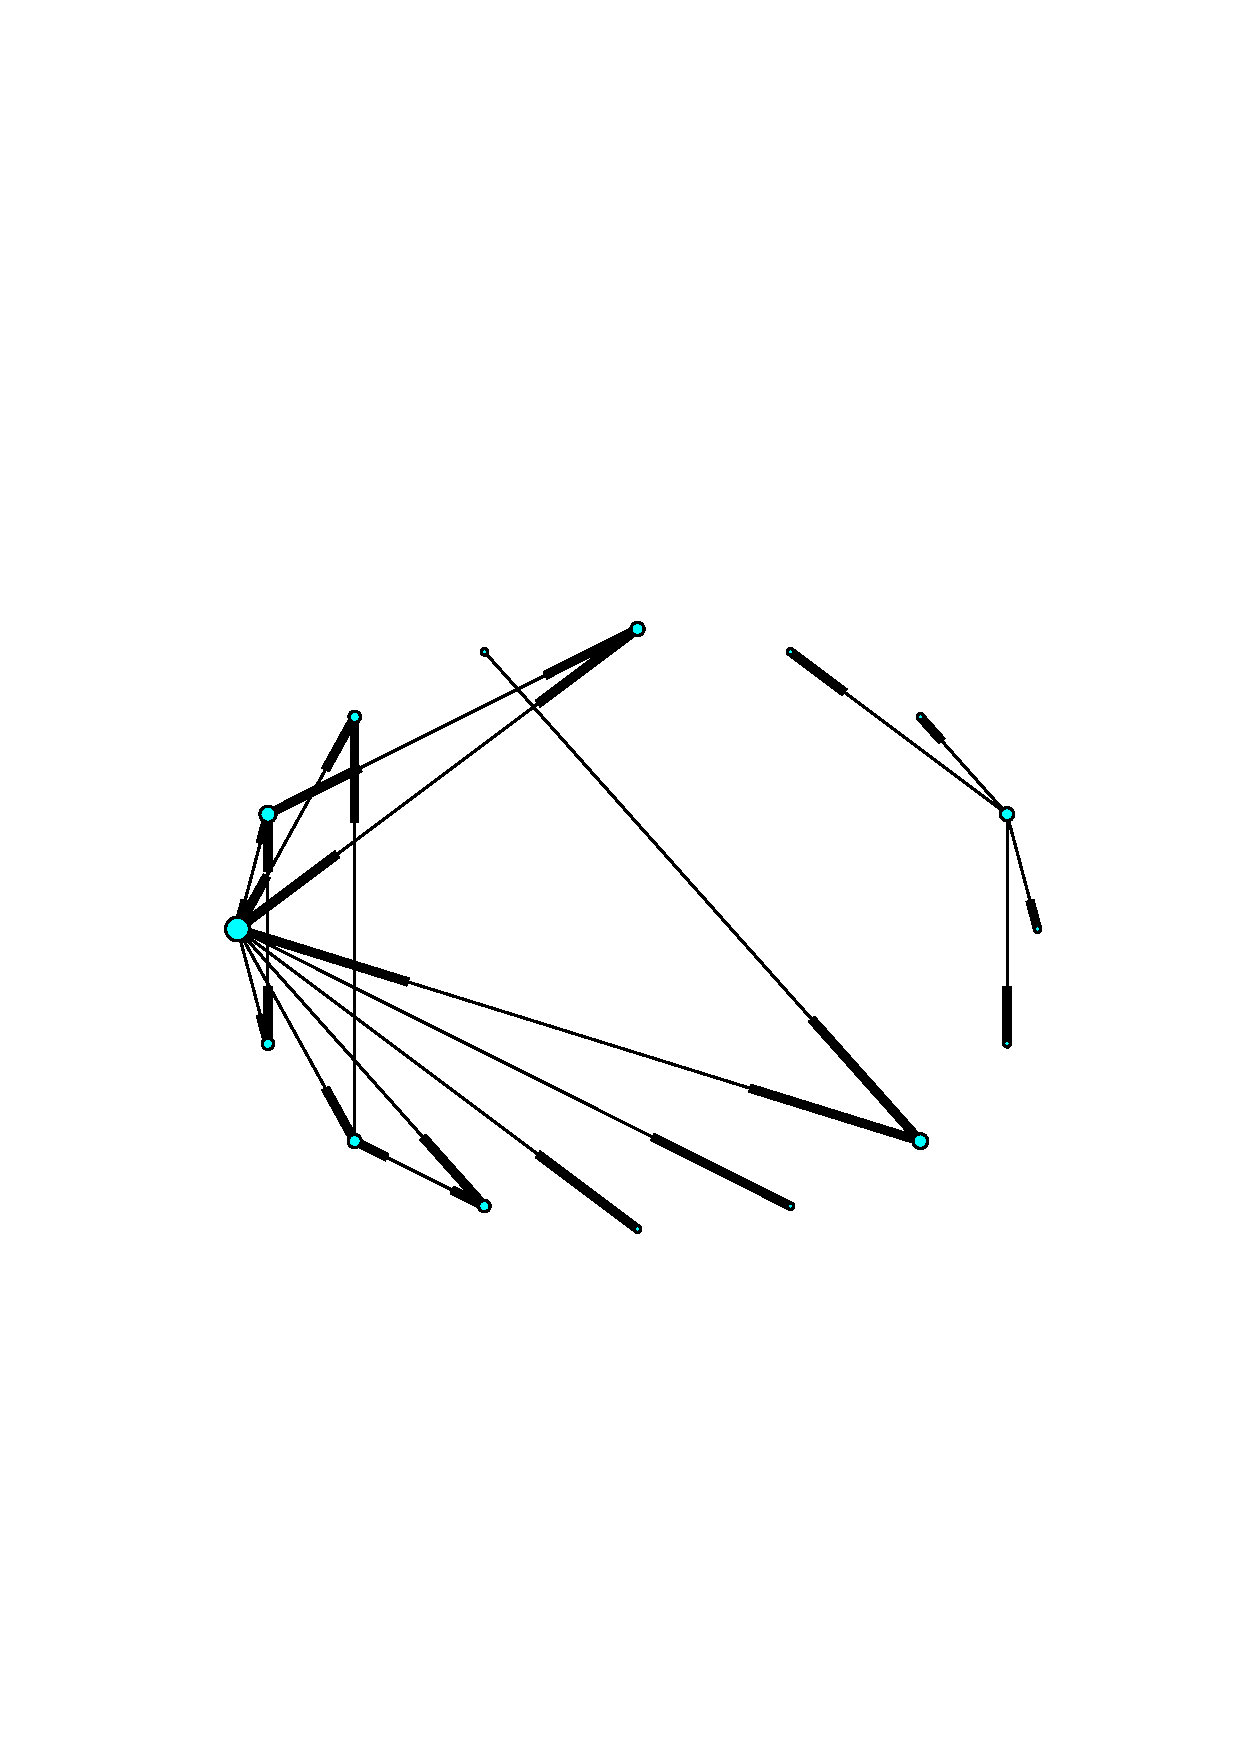
\includegraphics[width=\textwidth]{eth-red-domestica.png}

\subsubsection{Red corporativa de empresa de Telecomunicaciones - wireless LAN}


\section{Conclusiones}



\addtolength{\textheight}{-12cm}   % This command serves to balance the column lengths
                                  % on the last page of the document manually. It shortens
                                  % the textheight of the last page by a suitable amount.
                                  % This command does not take effect until the next page
                                  % so it should come on the page before the last. Make
                                  % sure that you do not shorten the textheight too much.



%%%%%%%%%%%%%%%%%%%%%%%%%%%%%%%%%%%%%%%%%%%%%%%%%%%%%%%%%%%%%%%%%%%%%%%%%%%%%%%%

\begin{thebibliography}{99}

\bibitem{c1} http://www.wireshark.org
\bibitem{c2} http://www.secdev.org/projects/scapy/

\end{thebibliography}

\end{document}
